% !TeX spellcheck = lv_LV
\section{Klimats Latvijā}
%Enter antagonists. Mākoņi. Bloķē daudz saules apstarojuma. Cik LV mākoņainu dienu?
%Izanalizēt VTPMML meteo datus no 2013.
%Pajautāt Stasim kļūdas.

Saskaņā ar LU VTPMML klimatisko datu apkopojumu, kas parādīts \ref{fig:makoni_Riga}. att., mākoņainība Rīgā var sasniegt līdz 60\% jūlijā un līdz pat 90\% decembrī. Tas nozīmē, ka Saules paneļu efektivitātes novērtējumam Latvijas klimatā mākoņainība ir ļoti būtiska un tā palīdzēs prognozēt nepieciešamos enerģijas uzkrājumus un papildavotus, ja solārā enerģija tiek izmantota kā pamata enerģijas avots.
\begin{figure}[h]
	\centering
	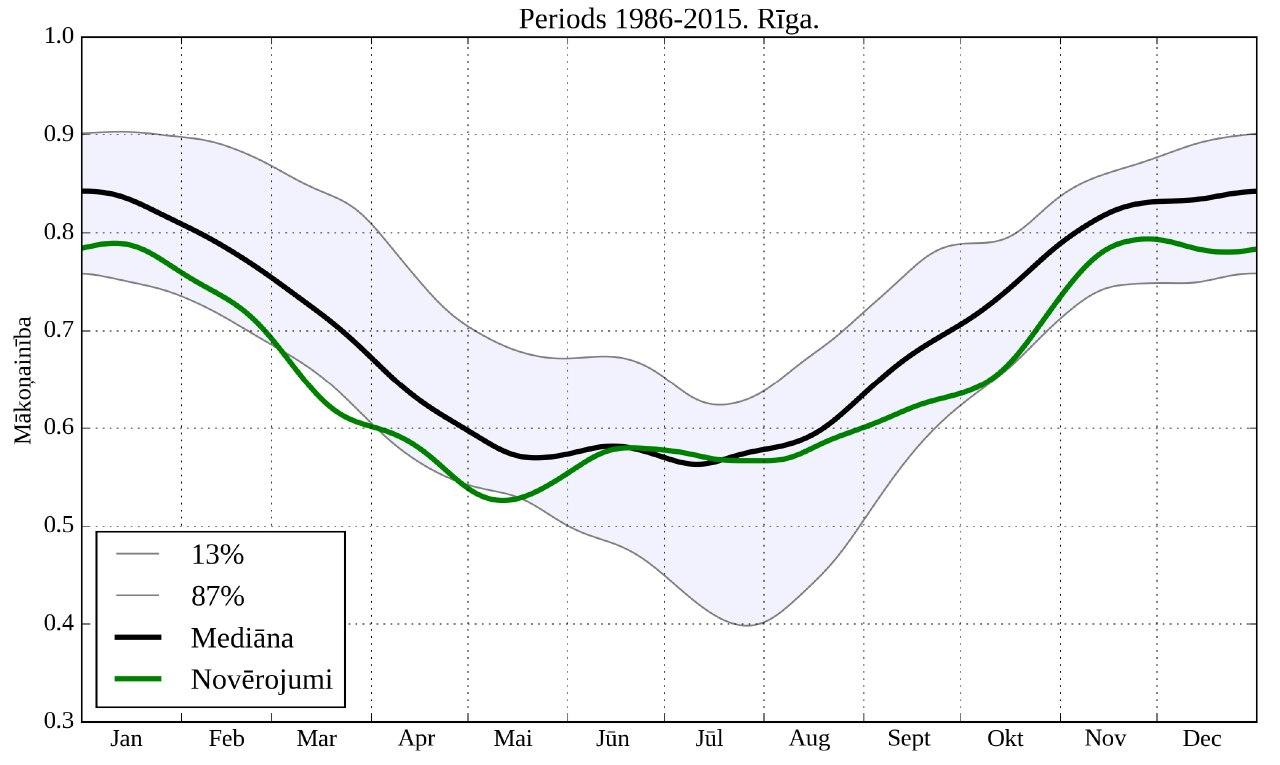
\includegraphics[width=0.8\linewidth]{figures/misc/makoni_riga.jpg}
	\caption{Vidējā mākoņainība Rīgā gada laikā, vidējota pa 20 gadu periodu~\cite{cloudsModlab}.}
	\label{fig:makoni_Riga}
\end{figure}

Mākoņu ietekme uz Saules apstarojumu ir komplicēta un atkarīga no dažādiem parametriem. Piemēram, pētījumā \cite{CloudCoverageImpactOnIrradiance} tiek parādīts, ka dažreiz mākoņainība var pat nedaudz palielināt Saules apstarojumu. Šis šķietami kontraintuitīvais rezultāts izskaidrojams ar to, ka Saule nav nosegta pilnībā, un baltie mākoņi mēdz būt gaišāki nekā pašas debesis saulainā dienā (sk. \ref{fig:makoni_ietekme}.(b) attēlā), tādējādi DNI komponentes samazināšanās tiek kompensēta ar palielinātu gaismas izkliedi. 

Savukārt gadījumos, kad mākoņi aizsedz Sauli (sk. \ref{fig:makoni_ietekme}.(c) attēlā), apstarojums $\approx99\%$ gadījumu samazinās, kā tas bija paredzams.
% Tomēr korelācija starp iegūto enerģiju un mākoņu daudzumu ir pat nedaudz pozitīva, kas atkal notiek palielinātas gaismas izkliedes dēļ. 
Apskatot visu datu kopu, var secināt, ka vairākumā gadījumu mākoņu ietekmi uz Saules paneļu saražoto enerģiju var uzskatīt par nelabvēlīgu. Tomēr pētījuma autori norāda, ka, neskatoties uz to, ka mākoņainība ir galvenais Saules paneļu efektivitāti ietekmējošs faktors, ar informāciju par mākoņainību nepietiek, lai pilnvērtīgi izskaidrotu un paredzētu paneļu saražotās enerģijas izmaiņas.

\begin{figure}[h]
	\centering
	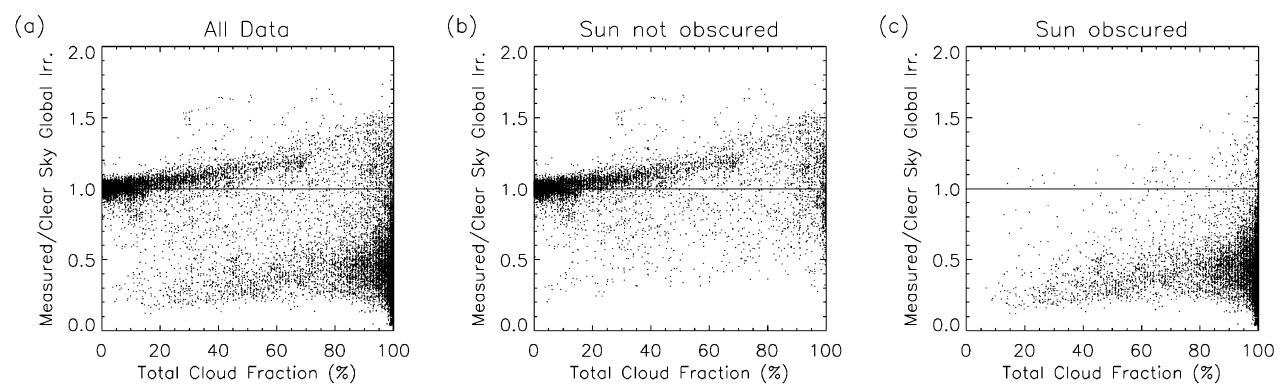
\includegraphics[width=\linewidth]{figures/misc/makoni_ietekme.jpg}
	\caption{Attiecība starp izmērīto apstarojumu un tīrās debess gadījuma apstarojumu (a) visiem datiem, (b) gadījumos ar neaizsegtu Sauli un (c) gadījumos ar aizsegtu Sauli~\cite{CloudCoverageImpactOnIrradiance}.}
	\label{fig:makoni_ietekme}
\end{figure}

Mākoņu ietekme ir atkarīga arī no to veida. Mākoņu modifikācijas reizinātājs (\textit{Cloud Modification Factor} - CMF), ko definē kā attiecību starp apstarojumu gadījumos ar un bez mākoņiem, atkarībā no mākoņu tipa ir apkopots \ref{tab:CMF}. tabulā. Ir jāņem vērā, ka CMF ir atkarīgs no viļņa garuma. Tomēr ultravioletais CMF no redzamās gaismas CMF ir atkarīgs lineāri ar koeficientiem $\approx0.6-1$ gubumākoņu gadījumā un eksponenciāli spalvmākoņu gadījumā.
\begin{table}[h]
	\caption{CMF intervāls atkarībā no mākoņu tipa~\cite{effectCloudsOnSurface}}
	\begin{center}
		\begin{tabular}{| r | c |}
			\hline
			augstie gubumākoņi & $<0.7$     \\ \hline
			gubumākoņi         & $0.2-1.3$ \\ \hline
			spalvmākoņi        & $0.6-1$    \\ \hline
		\end{tabular}
	\end{center}
	\label{tab:CMF}
\end{table}

Mākoņu ietekmes uz Saules apstarojumu modelēšana ir ļoti sarežģīta. Mērījumi parāda, ka mākoņi absorbē par 25 W/m$^2$ vairāk gaismas, nekā teorētiski paredzams, un šī vērtība nevar būt izskaidrojama ar troposfēras aerosoliem ~\cite{observVSModel}.
% Sekmīgajai modeļa darbībai ir nepieciešama parametru verifikācija, ko ir grūti veikt mazāk attīstītās valstīs, kur eksperimentālo datu skaits nav tik izsmeļošs, kā attīstītajās valstīs. Šādos apstākļos statistiska pieeja (piemēram, iepriekš iegūto klimatisko datu vidējošana un ekstrapolēšana) var izrādīties vienkāršāka un dažreiz pat precīzāka par matemātiskajiem modeļiem [shorturl.at/mDNT3]. Papildus grūtības rada arī tas, ka Saules apstarojums svārstās Saules aktivitātes ciklu dēļ. Tomēr šā darba ietvaros to var neņemt vērā salīdzinoši nelielas ietekmes dēļ, jo GHI mainās tikai ap 0.7~W/m$^2$ gadā
% [changes\_of\_solar\_radiation\_at\_earth\_surface.pdf].